\documentclass[addpoints]{exam}
\usepackage[utf8]{inputenc}




\usepackage{pdfsync}
\usepackage{fontspec}
\usepackage[T1]{fontenc}
\usepackage[utf8]{inputenc}
\usepackage{etoolbox}
\usepackage{tikz}
\usepackage{pgfplots}
\usepackage{subfig}
\usepackage{tikzscale} % Scale the figure not the font
\tikzset{
font={\fontsize{5pt}{5}\selectfont}}
\usepackage{tikzscale} % Scale the figure not the font
\usepackage{textpos}
\usepackage{standalone}
\usepackage{color}
\pgfplotsset{tick scale binop=\times}
\usepackage{tikz-dimline}
\usepackage[skins,theorems]{tcolorbox}
\usepackage{animate}


\usepackage{amsmath}
\usepackage{booktabs}
\usepackage{cancel}
\usepackage{caption}
\usepackage{cleveref}
\usepackage{colortbl}
\usepackage{csquotes}
% \usepackage{helvet}
% \usepackage{millennial}
\usepackage{multirow}
\usepackage{listings}
\usepackage{xcolor}

\usepackage{esint} % various fancy integral symbols
\usepackage{outlines}



\usepackage{physics} % For using the oridnary derivative
\usepackage{siunitx}
\sisetup{per=slash, load=abbr, output-complex-root = j, complex-root-position = before-number, round-mode=figures,round-precision=4}

%% Tikz Libraries
\usetikzlibrary{positioning}
\usetikzlibrary{arrows}
\usetikzlibrary{patterns}
\usetikzlibrary{backgrounds}
\usetikzlibrary{calc}
\usetikzlibrary{decorations.pathreplacing}



\newcommand{\ti}[1]{\tilde{#1}} % spectral representation
\newcommand{\tnsr}[1]{\underline{\underline{#1}}}

% Symbols
\renewcommand{\O}{\omega}  % omega
\newcommand{\E}{\varepsilon}  % epsilon
\renewcommand{\u}{\mu}  % mu
\newcommand{\p}{\rho}  % rho
\newcommand{\x}{\times}  % times
\renewcommand{\inf}{\infty}  % infinity
\newcommand{\infint}{\int\limits_{-\inf}^\inf} % integral by R
\newcommand{\e}{\mathrm{e}} % Straight-up exponential
\renewcommand{\j}{{j}\mkern1mu} % Straight-up exponential
\newcommand{\iu}{\mathrm{i}\mkern1mu}

\newcommand\ddfrac[2]{\frac{\displaystyle #1}{\displaystyle #2}}

\title{High Frequency Communication Systems}
\author{Homework 5 - Transmission Lines and Smith Chart}
\date{Semester 2, 2020/21}

\begin{document}

\maketitle


\begin{questions}
    \pointsinrightmargin 
    \bracketedpoints
\question[3] A lossless transmission line of electrical length $\ell=0.3 \lambda$ is terminated with a complex load impedance as shown in the Figure \ref{fig:problem1}. Find the reflection coefficient at the load, the VSWR on the line, the reflection coefficient at the input of the line, as well as the input impedance of the line.

\begin{figure}[h!]
    \centering
    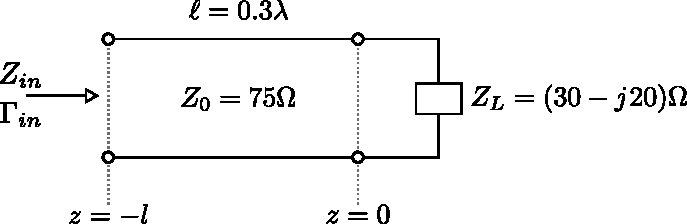
\includegraphics[width = 0.75\textwidth]{problem1.pdf}
    \caption{Problem 1 - Transmission Line.}
    \label{fig:problem1}
\end{figure}


\question[2] Let $Z_{SC}$ be the input impedance of a length of coaxial line when one end is short-circuited, and let $Z_{OC}$ be the input impedance of the line when one end is open-circuited. Derive an expression for the characteristic impedance of the cable in terms of $Z_{SC}$ and $Z_{OC}$.


\question[2]
For a purely reactive load impedance of the form $Z_{L}=\j X,$ show that the reflection coefficient magnitude $|\Gamma|$ is always unity. Assume that the characteristic impedance $Z_{0}$ is real.


\question
\begin{parts}
    \part[1]
    Why is it more convenient to use admittance on the Smith chart when dealing with impedance matching problems?
    \part[1]
    Why do we use short-circuit type stubs instead of open-circuit type for impedance matching?

    \part[1]
    Assess the advantages of double stub matching over single stub?
    \end{parts}

    \question[4]
    Design a double-stub tuner using open-circuited stubs with a $\lambda / 8$ spacing to match a load admittance $Y_{L}=(0.4+j 1.2) Y_{0}$.
\end{questions}
\end{document}

